\subsubsection{\texttt{RF-11}: sincronización automática de las modificaciones en los ejercicios durante su realización}
\label{subsec:rf11}

Dentro de la visualización del detalle de los cursos, una vez se ha seleccionado un directorio (\referenciaConTT{subsec:rf9}{RF-9}) y se ha descargado el estado de los ejercicios en progreso o se ha decidido utilizar la información previamente disponible en local (\referenciaConTT{subsec:rf10}{RF-10}), estos ejercicios comienzan a sincronizarse automáticamente con el servidor.

En lo que a la interacción con el usuario respecta, la interfaz muestra para cada ejercicio en progreso dos señales de activación de la sincronización automática y de su estado. La \referenciaFigura{fig:reqf11-1} refleja la visualización de los dos estados posibles: o bien la aplicación se encuentra esperando a que ocurran nuevos cambios y la sincronización del ejercicio está finalizada porque no hay nuevos cambios a comunicar al servidor (izquierda), o bien se está produciendo la transmisión al servidor de las modificaciones de uno o más ficheros (derecha). Los indicadores mostrados en esta figura quedan encuadrados dentro del estado de cada ejercicio.

\begin{figure}[ht]
    \centering
    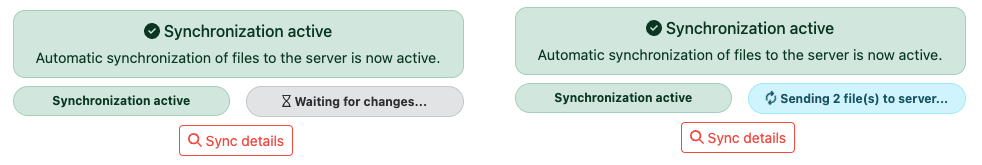
\includegraphics[width=0.9\textwidth]{imagenes/utilizadas/4-3-implementacion/rf11-1.png}
    \caption{Captura de las señales de sincronización activa y estado de la sincronización de ejercicios en progreso.}
    \label{fig:reqf11-1}
\end{figure}

El segundo elemento es el botón ``Sync details'' (detalles de la sincronización) que se muestra debajo del estado de la sincronización en cada ejercicio (visible en la \referenciaFigura{fig:reqf11-1}). Cuando se pulsa, se despliega un modal que contiene una lista con el histórico de los diez ficheros sincronizados más recientemente, los diez siguientes ficheros que serán sincronizados y el que está siendo transmitido al servidor en el momento presente, que dispone de una barra de progreso indicativa del avance de la operación.

La \referenciaFigura{fig:reqf11-2} muestra dos ejemplos de este modal: uno durante la sincronización de un fichero muy pesado (arriba) y otro que refleja la sincronización de una ingente cantidad de ficheros (abajo), constando de una lista de más de 150 ficheros sincronizados y de más de 300 ficheros pendientes de sincronizar. Para cada fichero sincronizado o pendiente de subir, se incluyen dos iconos: uno para reflejar el estado de la subida (rojo si está pendiente, amarillo si está en progreso y verde si se finalizó) y otro que indica el tipo de sincronización, pudiendo tratarse de la creación de un fichero (verde), una modificación de un fichero previamente existente (amarillo) o una eliminación (rojo). Los renombramientos aparecen como eliminaciones y nuevas creaciones.

\begin{figure}[ht]
    \centering
    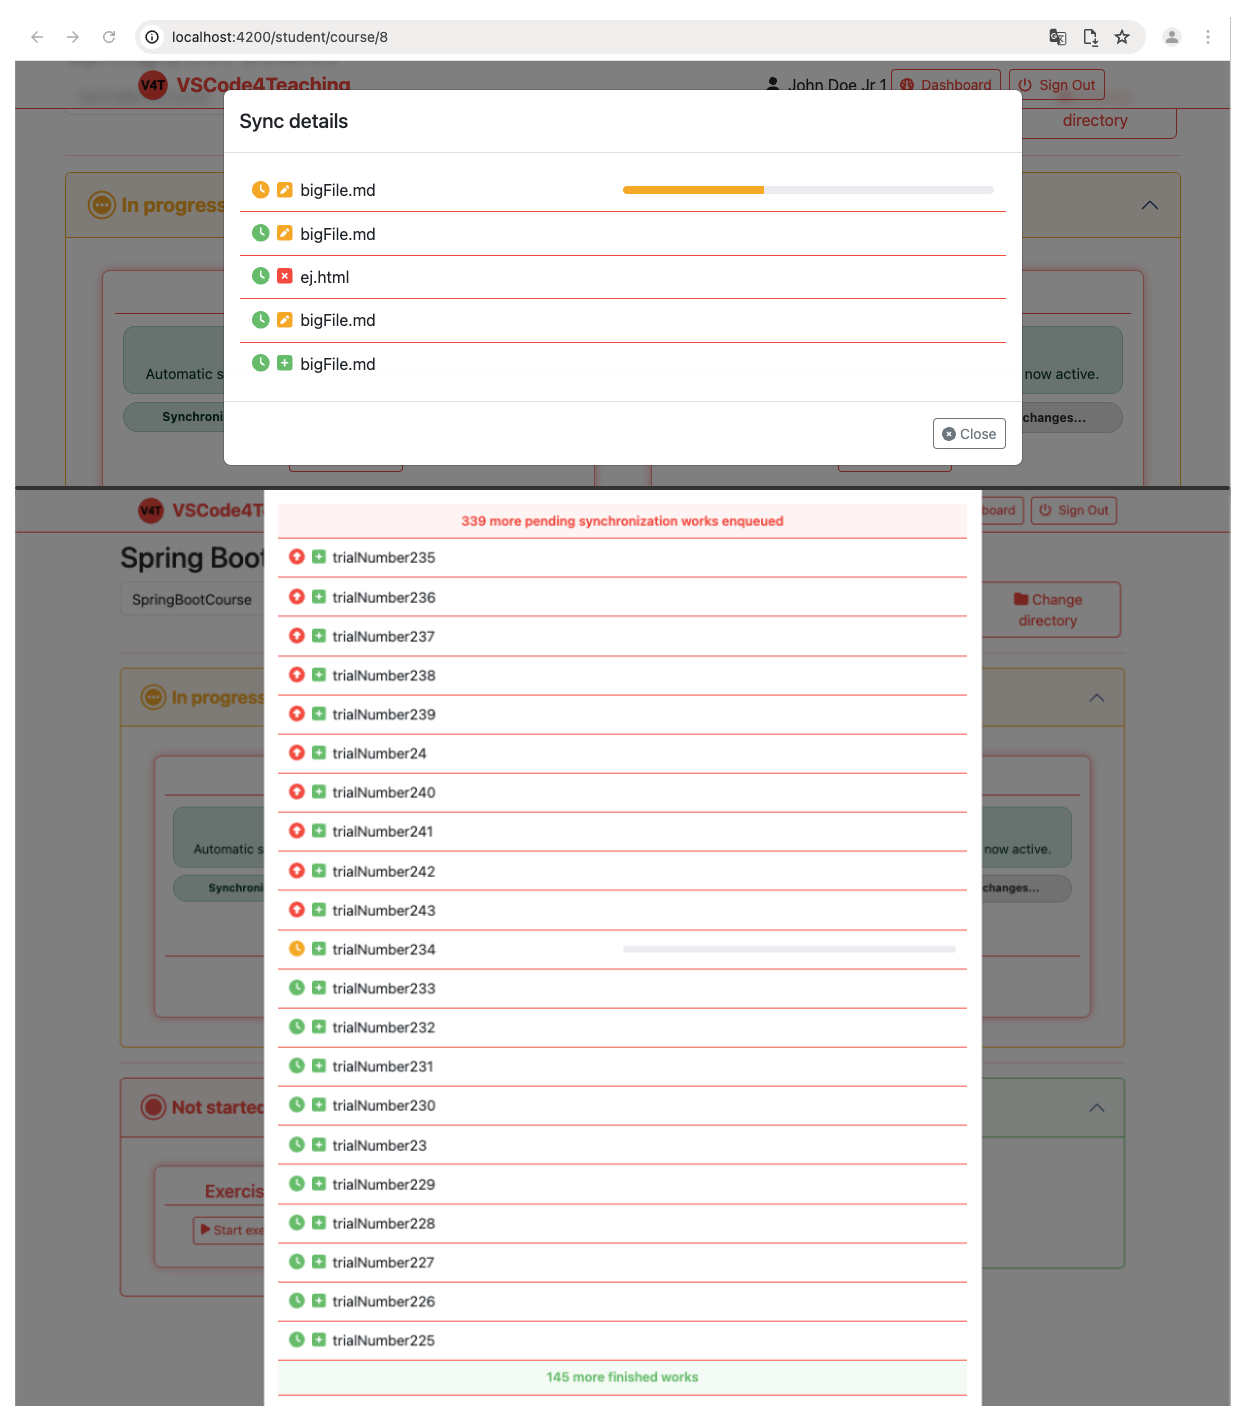
\includegraphics[width=0.8\textwidth]{imagenes/utilizadas/4-3-implementacion/rf11-2.png}
    \caption{Captura del modal explicativo de la sincronización de ficheros de un ejercicio.}
    \label{fig:reqf11-2}
\end{figure}

El diseño e implementación del algoritmo destinado a los procesos automáticos de cotejamiento y sincronización de cada ejercicio en progreso queda desarrollado pormenorizadamente en el \referenciaAnexo{anx:bajoNivelRF11}.
